\chapter{Theory}
\section{Coverage Path Planning and Lawnmower Patterns}

Coverage path planning addresses the problem of generating trajectories that systematically visit all locations within a defined workspace. The objective is to ensure no areas remain uninspected while minimizing redundant coverage and maintaining efficient operation \cite{galceran2013survey}. 

Among various CPP approaches, the boustrophedon pattern has gained widespread adoption in robotics. This method structures the coverage task as a series of parallel, straight-line transects connected by turning maneuvers at the workspace boundaries\cite{choset1998coverage, choset2000coverage}. The pattern is shown in \ref{fig:boustrophedon}

The lawnmower pattern exhibits favorable computational characteristics compared to alternative CPP methods. Path generation requires only geometric calculations based on workspace dimensions and sensor parameters, avoiding iterative optimization or graph search algorithms.\cite{choset2000coverage}. The approach provides completeness guarantees for convex workspaces.\cite{choset1998coverage}.


The fundamental geometric parameter governing coverage completeness is the spacing between parallel tracks. Consider a sensor with effective detection width $d_{\text{sensor}}$. To guarantee that no regions remain unobserved, adjacent tracks must be spaced such that:
\begin{equation}
d_{\text{track}} \leq d_{\text{sensor}}
\end{equation}

In practice, perfect path following rarely occurs due to environmental disturbances, vehicle dynamics, and positioning errors. To maintain coverage reliability under these real-world conditions, an overlap factor is introduced:
\begin{equation}
d_{\text{track}} = (1 - \alpha) \cdot d_{\text{sensor}}, \quad \alpha \in [0.1, 0.3]
\end{equation}
where $\alpha$ represents the fractional overlap between adjacent sensor footprints \cite{galceran2013survey}. Typical values range from 10\% to 30\% depending on positioning accuracy and mission criticality.

\begin{figure}[t]
    \centering
    % Requires: \usepackage{tikz}
    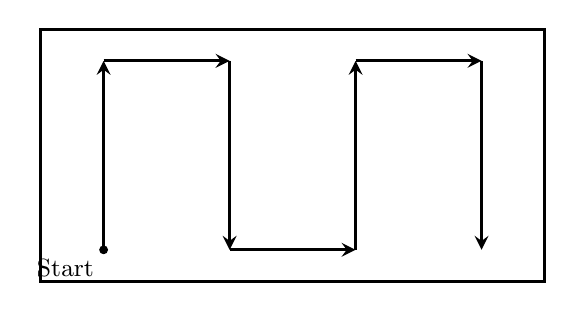
\begin{tikzpicture}[scale=0.8, >=stealth]

        % Workspace boundary
        \draw[very thick] (0,0) rectangle (8,4);



        % Connected single-pass path (one sweep per cell)
        % Cell 1
        \draw[very thick,->] (1,0.5) -- (1,3.5);
        % Move to Cell 2
        \draw[very thick,->] (1,3.5) -- (3,3.5);
        % Cell 2
        \draw[very thick,->] (3,3.5) -- (3,0.5);
        % Move to Cell 3
        \draw[very thick,->] (3,0.5) -- (5,0.5);
        % Cell 3
        \draw[very thick,->] (5,0.5) -- (5,3.5);
        % Move to Cell 4
        \draw[very thick,->] (5,3.5) -- (7,3.5);
        % Cell 4
        \draw[very thick,->] (7,3.5) -- (7,0.5);

 

        % Start marker
        \fill (1,0.5) circle (2pt);
        \node[below left] at (1,0.5) {\small Start};

    \end{tikzpicture}
    \caption{boustrophedon style coverage path.}
    \label{fig:boustrophedon}
\end{figure}




\section{Pure Pursuit Guidance}

Pure Pursuit is a geometric path-following algorithm that steers the vehicle toward a lookahead point on the desired path \cite{fossen2021handbook}. Given vehicle position $\mathbf{p} \in \mathbb{R}^2$ and path waypoints $\{\mathbf{w}_1, \ldots, \mathbf{w}_N\}$, the algorithm selects target point $\mathbf{p}_d$ at a lookahead distance along the path and computes the desired velocity:
\begin{equation}
\mathbf{v}_d = k_g \frac{\mathbf{p}_d - \mathbf{p}}{\|\mathbf{p}_d - \mathbf{p}\|}
\end{equation}
where $k_g > 0$ determines approach speed.

\section{Sliding Variables in Control}
\begin{quote}
    Hva skal jeg skrive her??? Må fine ut om definisjonen skal her eller i metode
\end{quote}
A sliding variable is a scalar or vector function that combines tracking errors with their temporal derivatives or integrals to achieve desired closed-loop dynamics \cite{slotine1991applied}. Rather than controlling each error component independently, the sliding variable formulation reduces the control problem to driving a single composite variable to zero.

For a tracking problem with position error $\mathbf{e} = \mathbf{p} - \mathbf{p}_d$, a sliding variable incorporating integral action takes the form:
\begin{equation}
\boldsymbol{\sigma} = \mathbf{e} + \lambda \int_0^t \mathbf{e}(\tau) \, d\tau
\end{equation}
where $\lambda > 0$ is a design parameter. When the sliding variable reaches zero ($\boldsymbol{\sigma} = \mathbf{0}$), the system exhibits first-order error dynamics $\dot{\mathbf{e}} = -\lambda \mathbf{e}$, ensuring exponential convergence to the desired trajectory. The integral term provides steady-state error elimination in the presence of constant disturbances, making this formulation particularly effective for systems subject to persistent external forces such as ocean currents or wind.



\section{Switching Control}

Switching control refers to feedback laws in which a plant is regulated by selecting among multiple controllers according to a discrete switching signal. Liberzon characterizes switched control systems as continuous dynamical systems whose evolution is governed by ``continuous dynamics with isolated discrete switching events'' \cite[p.~3]{liberzon2003switching}. The closed-loop system consists of several continuous subsystems,
\begin{equation}
\dot{x} = f_i(x), \qquad i \in \mathcal{M},
\end{equation}
and a switching law $\sigma(t)$ determining the active mode:  
\begin{equation}
\dot{x} = f_{\sigma(t)}(x).
\end{equation}

\subsection*{State-Dependent Switching in Continuous Systems}
Switching signals may depend on the system state. Liberzon defines this as \emph{state-dependent switching}, where transitions occur when $x(t)$ enters a region or crosses a ``switching surface'' separating the domains of different subsystems \cite[p.~5]{liberzon2003switching}. These switching surfaces partition the continuous state space, and the dynamics may switch when
\[
x(t) \in S_{ij} \;\Rightarrow\; \sigma(t^+) = j,
\]
with $S_{ij}$ denoting the boundary between subsystem $i$ and $j$.



\subsection*{Motivation for Switching Control}
Liberzon identifies specific scenarios where switching among continuous controllers is necessary \cite[p.~75]{liberzon2003switching}:
\begin{itemize}
    \item When the task inherently consists of several qualitatively different continuous behaviors, making a single feedback law unsuitable.
    \item When sensing or actuation constraints do not permit a continuous controller valid across all operating conditions.
    \item When system uncertainty or structural properties make global stabilization by a single continuous controller impossible.
\end{itemize}
Under such conditions, switching control provides a principled mechanism for achieving desired performance and stability by combining multiple continuous controllers within one hybrid closed-loop framework.

\begin{quote}
    argumenter for at dette er riktig men skal det her:::?
The system falls under all 3 categories:
1. "if the desired system trajectory is composed of entirely different types", we want to control different parameters in the moving directions, which warrants the desired behaviour of a switching controller.
2. Sensor limitations due to discrete measurements of top and bottom which is not known beforehand

Må redigere til å bare ta med matten jeg har tenkt til å bruke her
\end{quote}


\section{PID Control}
PID control provides robust control for individual degrees of freedom. For error $e(t) = r(t) - y(t)$, the control law is:
\begin{equation}
u(t) = K_p e(t) + K_i \int_0^t e(\tau) \, d\tau + K_d \dot{e}(t)
\end{equation}
where $K_p$, $K_i$, and $K_d$ provide proportional, integral, and derivative action. 

The controller can be tuned by pole placement by setting the natural frequency $\omega_{n,i}$ and damping ratio $\zeta_i$, and time constant $T_i$, the gains are:
\begin{equation}
K_{p,i} = m_i \omega_{n,i}^2, \quad K_{d,i} = 2 m_i \zeta_i \omega_{n,i} \quad K_{i,i}=K\frac{K_{p,i}}{T_{i,i}}
\end{equation}


\subsection{Anti-Windup}
Anti-windup strategies prevent integral buildup during saturation or large transients. this is an undesirable effect and can be counteracted by clamping it to a maximum, or zeroing off in new states.
´